 % 若使用子图
% \graphicspath{{figs/}{headline_plots/}{appendix_plots/}}

% =========================
% Appendix — Supplementary Figures
% =========================
\appendix
\chapter{Supplementary Material}\label{Appendix:Figures}

This appendix collects supplementary tables and plots.
\begin{table}[t] \centering \caption{Investable universe (72 assets): full names and tickers. The anchor asset is BTC (No.\ 61).}
 \label{tab:assets} \scriptsize \setlength{\tabcolsep}{4pt} \renewcommand{\arraystretch}{1.05} \begin{tabularx}{\textwidth}{ r >{\raggedright\arraybackslash}X l r >{\raggedright\arraybackslash}X l r >{\raggedright\arraybackslash}X l} \toprule No. & Currency & Ticker & No. & Currency & Ticker & No. & Currency & Ticker \\ \midrule 1 & Oasis Network & \texttt{ROSE} & 25 & Tezos & \texttt{XTZ} & 49 & BNB & \texttt{BNB} \\ 2 & Ankr & \texttt{ANKR} & 26 & Loopring & \texttt{LRC} & 50 & Uniswap & \texttt{UNI} \\ 3 & VeChain & \texttt{VET} & 27 & Harmony & \texttt{ONE} & 51 & Stacks & \texttt{STX} \\ 4 & NEAR Protocol & \texttt{NEAR} & 28 & Solar & \texttt{SXP} & 52 & THORChain & \texttt{RUNE} \\ 5 & Ethereum & \texttt{ETH} & 29 & Kava & \texttt{KAVA} & 53 & Theta Network & \texttt{THETA}\\ 6 & EOS & \texttt{EOS} & 30 & Axie Infinity & \texttt{AXS} & 54 & Holo & \texttt{HOT} \\ 7 & BakeryToken & \texttt{BAKE} & 31 & Cardano & \texttt{ADA} & 55 & 1inch & \texttt{1INCH}\\ 8 & The Graph & \texttt{GRT} & 32 & Solana & \texttt{SOL} & 56 & Fetch.ai & \texttt{FET} \\ 9 & Reef & \texttt{REEF} & 33 & Ontology & \texttt{ONT} & 57 & Kusama & \texttt{KSM} \\ 10 & Injective & \texttt{INJ} & 34 & Ethereum Classic & \texttt{ETC} & 58 & Smooth Love Potion & \texttt{SLP} \\ 11 & Filecoin & \texttt{FIL} & 35 & Decentraland & \texttt{MANA} & 59 & Curve DAO Token & \texttt{CRV} \\ 12 & Polygon & \texttt{MATIC} & 36 & Synthetix & \texttt{SNX} & 60 & IoTeX & \texttt{IOTX} \\ 13 & Bitcoin Cash & \texttt{BCH} & 37 & Zcash & \texttt{ZEC} & 61 & Bitcoin & \texttt{BTC} \\ 14 & IOST & \texttt{IOST} & 38 & Conflux & \texttt{CFX} & 62 & Avalanche & \texttt{AVAX} \\ 15 & Chromia & \texttt{CHR} & 39 & Yearn Finance & \texttt{YFI} & 63 & Enjin Coin & \texttt{ENJ} \\ 16 & MultiversX & \texttt{EGLD} & 40 & Waves & \texttt{WAVES} & 64 & PancakeSwap & \texttt{CAKE} \\ 17 & Hedera & \texttt{HBAR} & 41 & Litecoin & \texttt{LTC} & 65 & XRP & \texttt{XRP} \\ 18 & Zilliqa & \texttt{ZIL} & 42 & Chiliz & \texttt{CHZ} & 66 & TRON & \texttt{TRX} \\ 19 & Algorand & \texttt{ALGO} & 43 & Stellar & \texttt{XLM} & 67 & Cosmos & \texttt{ATOM} \\ 20 & Dent & \texttt{DENT} & 44 & COTI & \texttt{COTI} & 68 & Aave & \texttt{AAVE} \\ 21 & Dash & \texttt{DASH} & 45 & Polkadot & \texttt{DOT} & 69 & Dogecoin & \texttt{DOGE} \\ 22 & My Neighbor Alice & \texttt{ALICE} & 46 & OMG Network & \texttt{OMG} & 70 & Neo & \texttt{NEO} \\ 23 & IOTA & \texttt{IOTA} & 47 & SushiSwap & \texttt{SUSHI} & 71 & The Sandbox & \texttt{SAND} \\ 24 & Chainlink & \texttt{LINK} & 48 & Fantom & \texttt{FTM} & 72 & Qtum & \texttt{QTUM} \\ \bottomrule \end{tabularx} \end{table}

% ---------- A. Distribution of monthly returns ----------
\begin{figure}[t]
\centering
% 推荐:把图保存为 appendix_plots/monthly_return_distribution.png
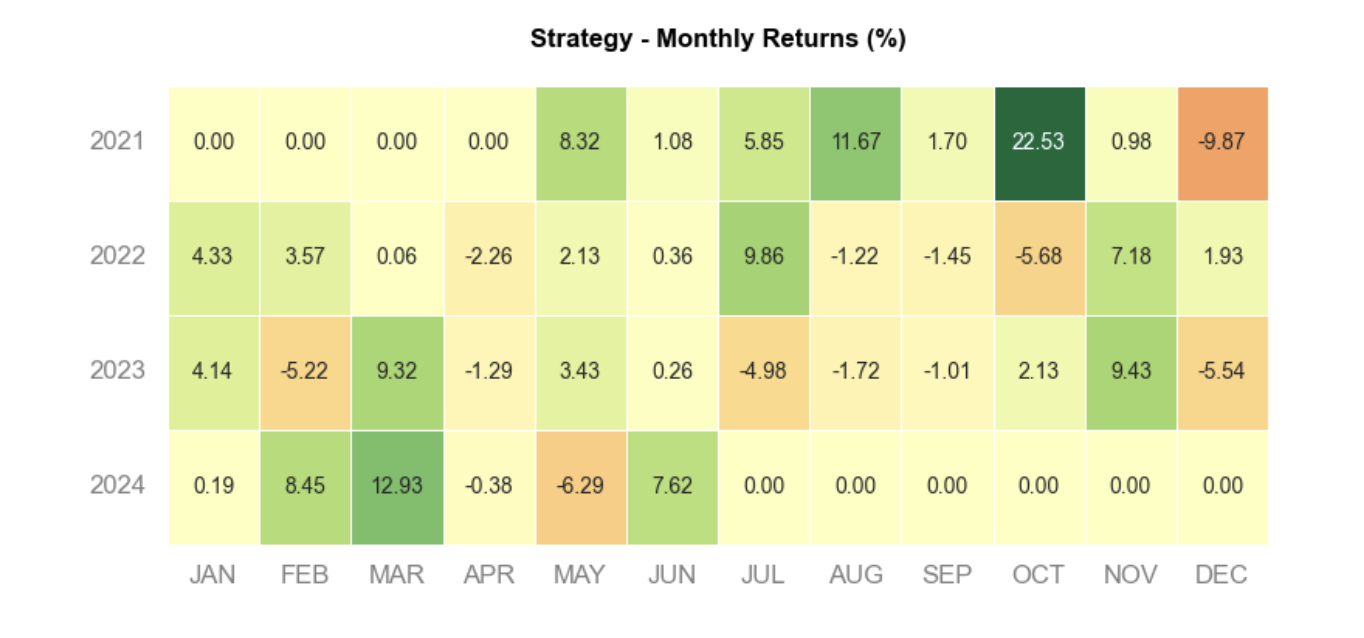
\includegraphics[width=0.92\linewidth]{headline_plots/monthly_return_distribution.png}
\caption{Distribution of monthly returns for the Baseline and the Strategy. Bars use common bins; the smooth lines are kernel density estimates. The Strategy shifts the mass to the right and trims the left tail relative to the Baseline.}
\label{fig:app:monthly_dist}
\end{figure}

% ---------- B. Underwater (drawdown) plot ----------
\begin{figure}[t]
\centering
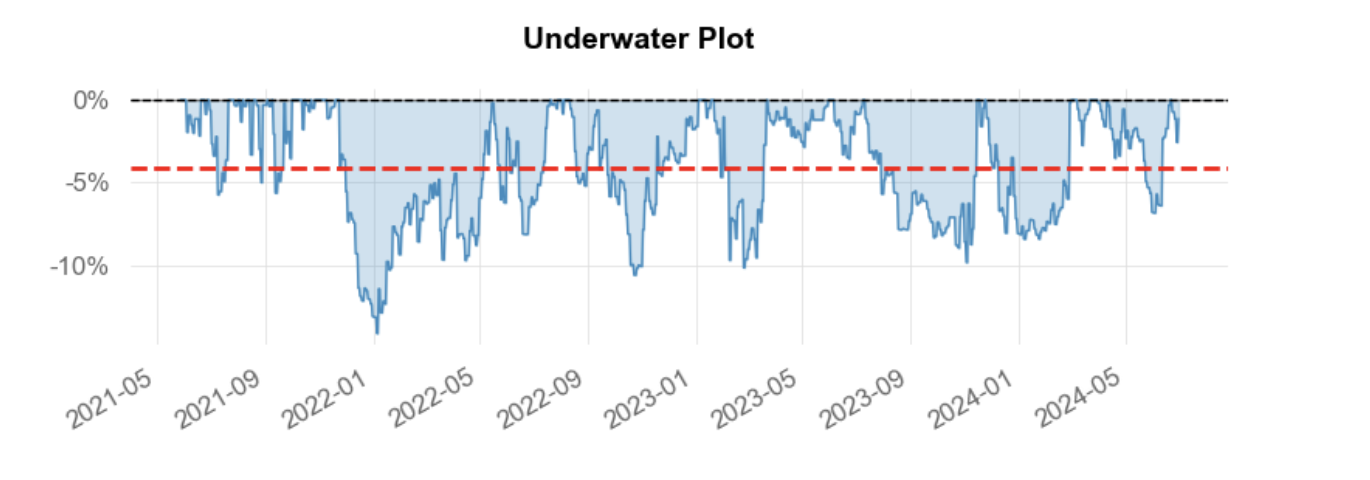
\includegraphics[width=0.95\linewidth]{headline_plots/underwater_plot.png}

\caption{Underwater plot (peak-to-trough drawdown over time) for the Strategy. The dashed line marks --5\%. The series shows clustered losses in early 2022 and faster recoveries thereafter, consistent with the overlay's regime-aware routing.}
\label{fig:app:underwater}
\end{figure}

% ---------- C. Monthly return heatmap ----------
\begin{figure}[t]
\centering
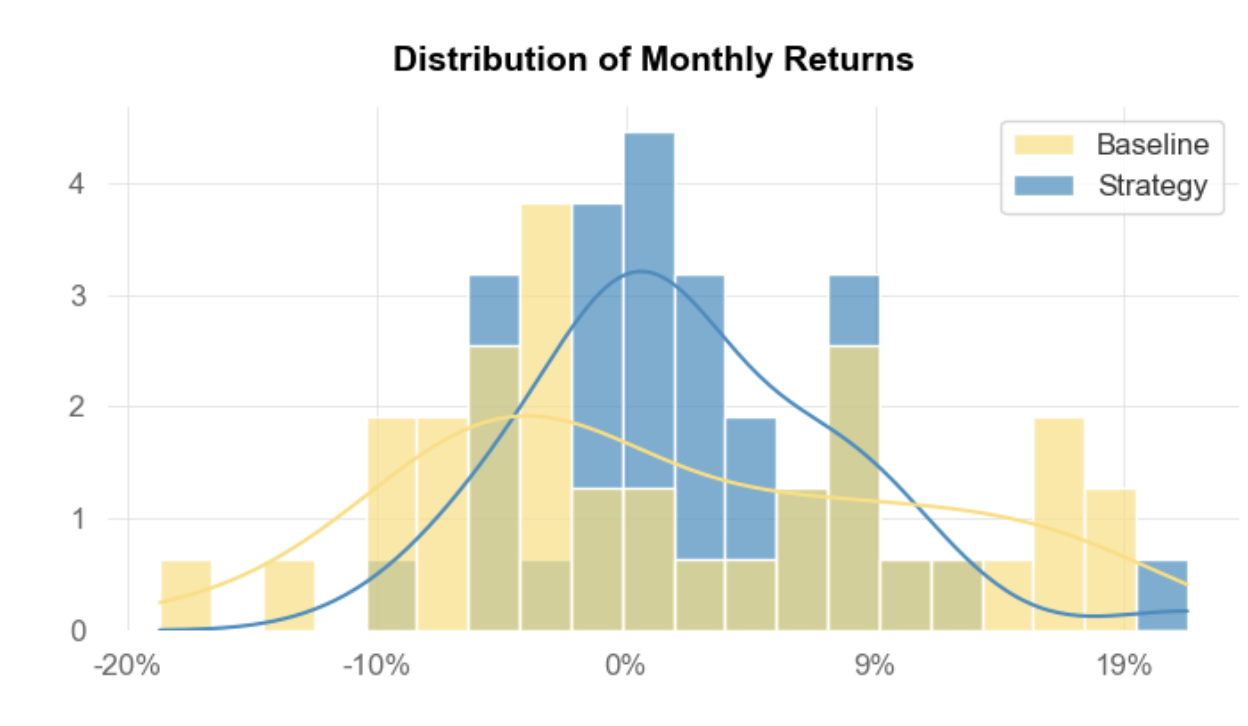
\includegraphics[width=0.98\linewidth]{headline_plots/monthly_returns_heatmap.png}

\caption{Monthly returns (\%) for the Strategy by calendar month. The heatmap highlights strong months in 2021Q4 and 2024Q1, as well as mixed outcomes during the 2022 drawdown.}
\label{fig:app:monthly_heatmap}
\end{figure}

% ---------- E. Switch-rate diagnostics ----------
\begin{figure}[t]
\centering
\includegraphics[width=\linewidth]{headline_plots/switches_per_year_top5.png}
% 备用:若不重命名,使用下行(包含空格/逗号/括号)
% \includegraphics[width=\linewidth]{\detokenize{/mnt/data/switches_per_year_top5.png}}
\caption{Switch-rate diagnostics for the top-5 parameterisations. 
Bars show the average number of basket switches per calendar year (signal on $t$, execution on $t^+$). 
Higher switch rates imply higher turnover and stronger cost sensitivity.}
\label{fig:app:switchrate_top5}
\end{figure}

% --- Regime timelines by parameter (no subfigure; one figure per page) ---


\begin{figure}[p]
  \centering
  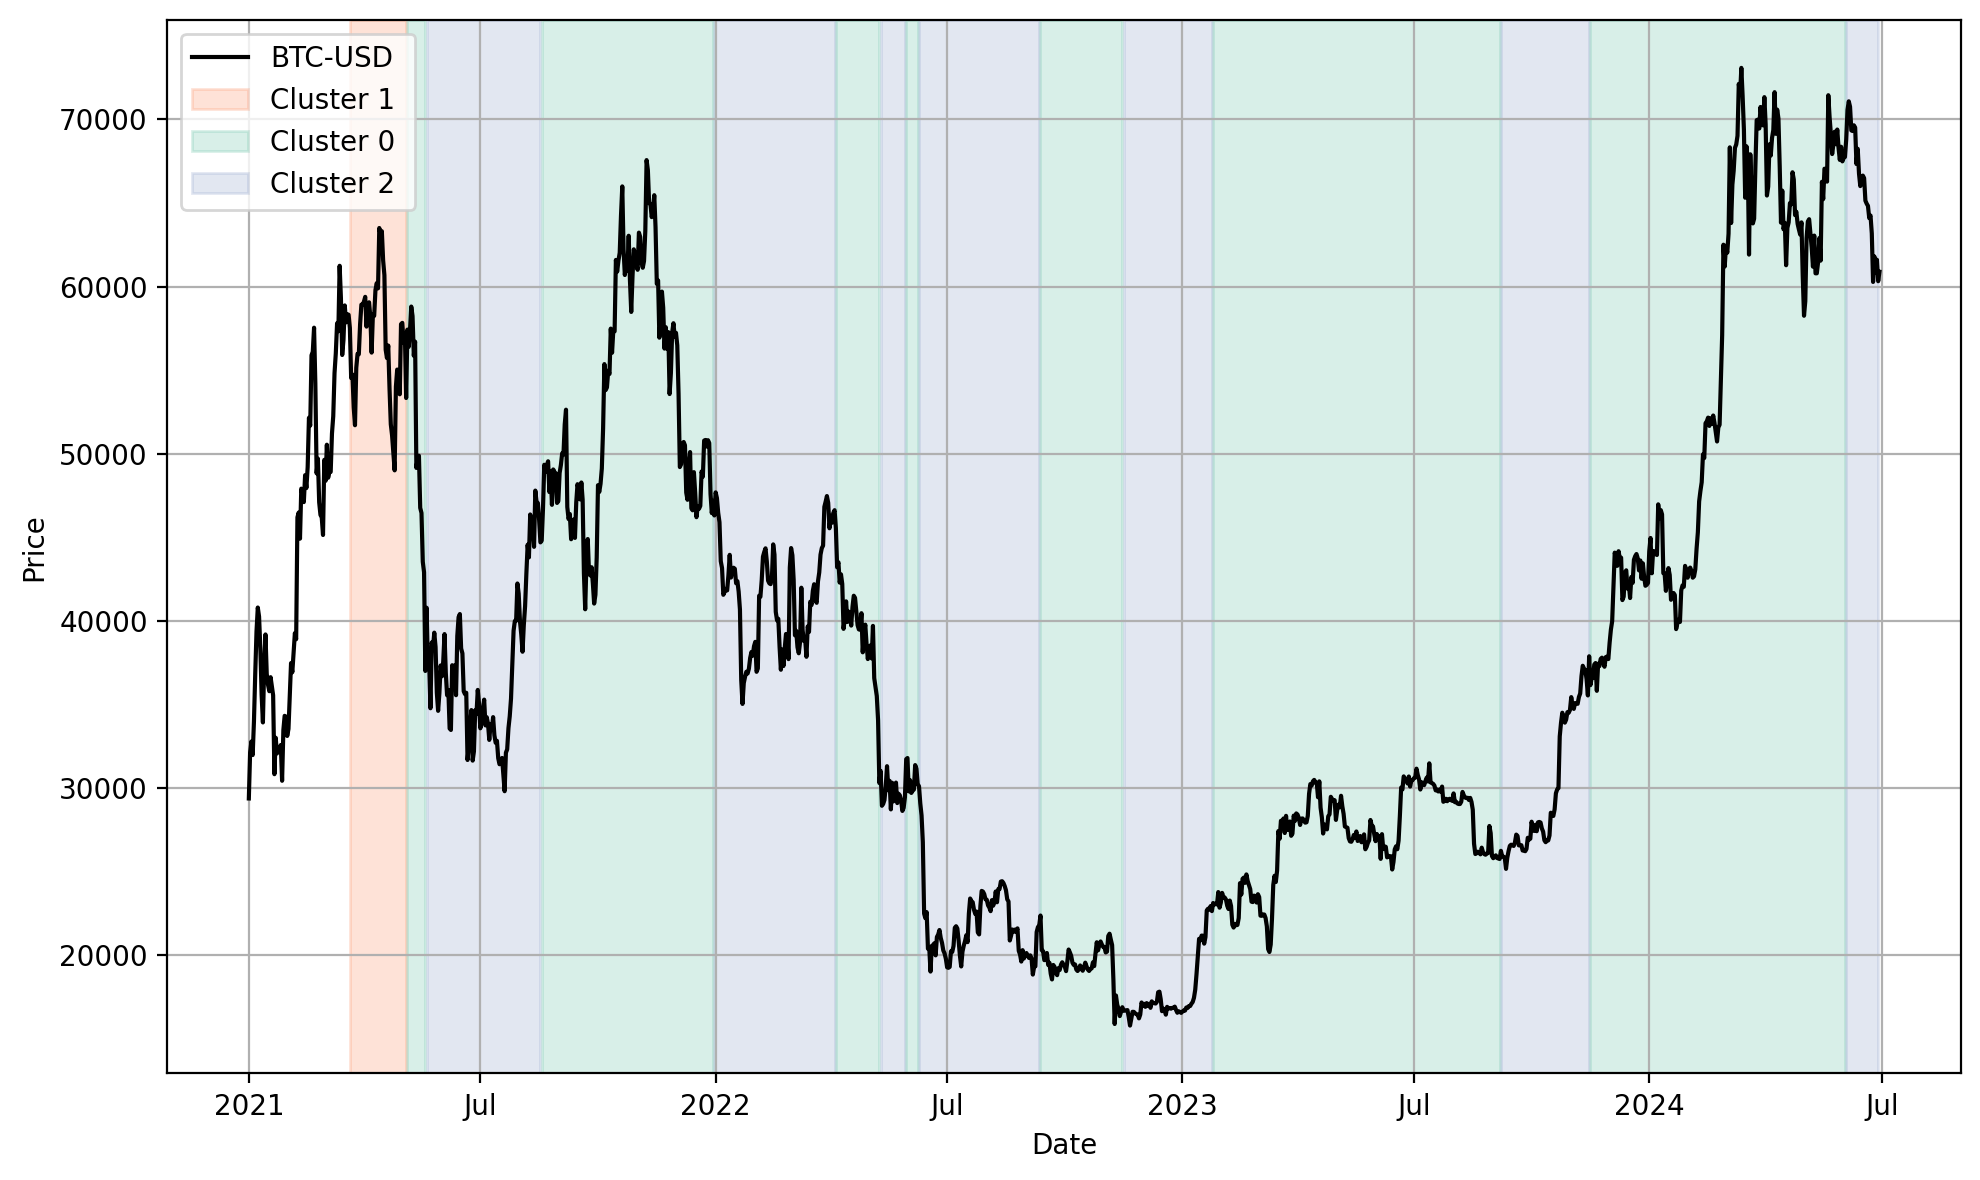
\includegraphics[width=\linewidth]{\detokenize{headline_plots/steps=5, paths=16, offset=0 (H=30, k=5, train_end=2023-07-05).png}}
  \caption{BTC price with walk–forward regime shading ($n_{\text{steps}}{=}5$, $n_{\text{paths}}{=}16$; $H{=}30$, $k{=}5$, $o{=}0$).}
  \label{fig:reg_s5_p16}
\end{figure}

\begin{figure}[p]
  \centering
  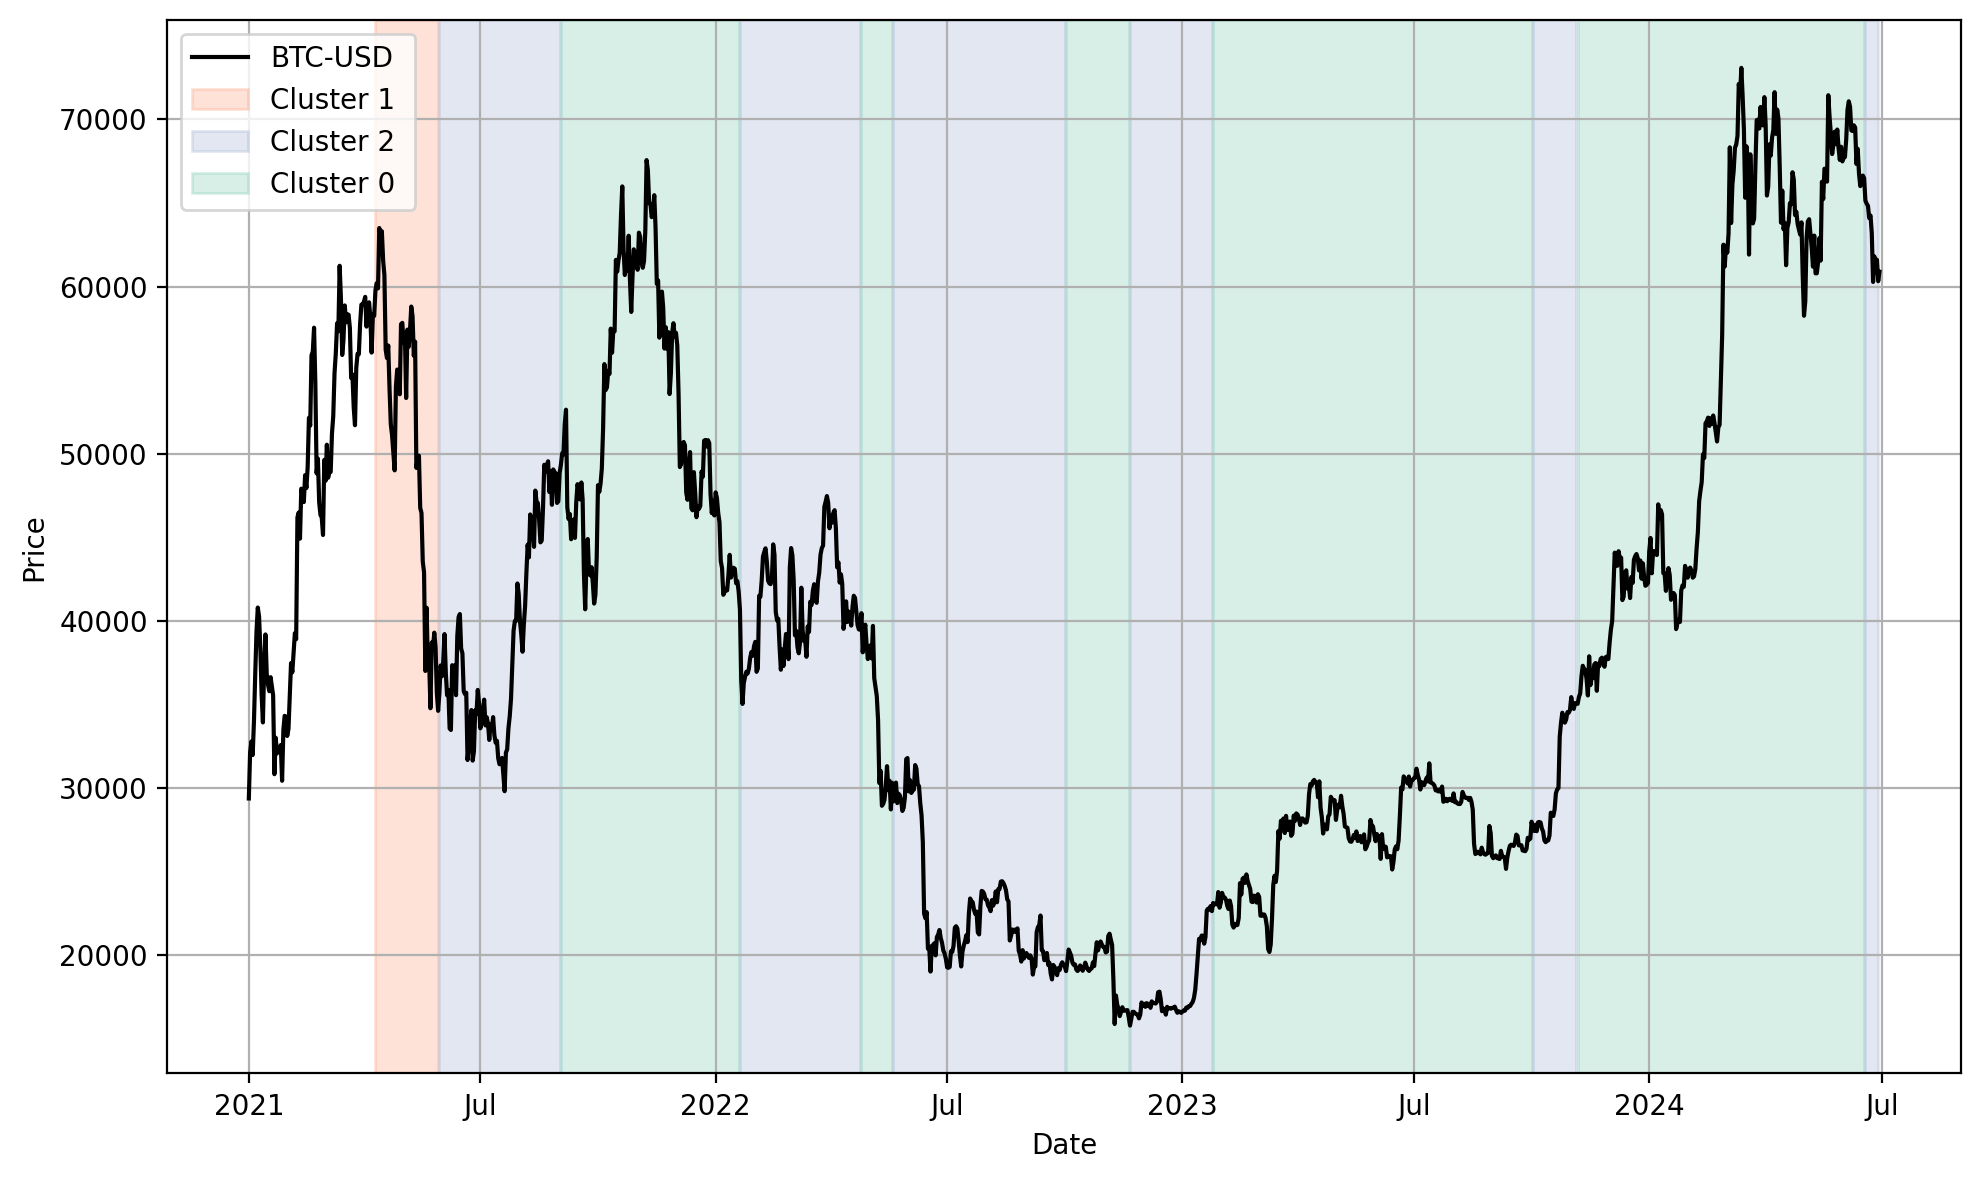
\includegraphics[width=\linewidth]{\detokenize{headline_plots/steps=5, paths=20, offset=0 (H=30, k=5, train_end=2023-07-11).png}}
  \caption{BTC price with walk–forward regime shading ($n_{\text{steps}}{=}5$, $n_{\text{paths}}{=}20$; $H{=}30$, $k{=}5$, $o{=}0$). Increasing the number of paths stabilises the state sequence and shortens spurious flips.}
  \label{fig:reg_s5_p20}
\end{figure}

\begin{table}[t]
\centering
\caption{White’s Reality Check (WRC) and Hansen’s SPA (overall $p=0.6645$). Mean differences are daily (overlay $-$ baseline).}
\label{tab:wrc_spa}
\small
\begin{tabular}{lrrrrr}
\toprule
Strategy $(n_{\text{steps}},n_{\text{paths}})$ & WRC mean\_diff & WRC (bp/day) & SPA mean\_diff & SPA std & Rank (WRC) \\
\midrule
(5, 20) &  0.000033 &  0.33 &  0.000033 & 0.015737 & 1 \\
(5, 16) & -0.000140 & -1.40 & -0.000140 & 0.013985 & 2 \\
(5,  8) & -0.000298 & -2.98 & -0.000298 & 0.015934 & 3 \\
(15,16) & -0.000340 & -3.40 & -0.000340 & 0.017153 & 4 \\
(15,12) & -0.000366 & -3.66 & -0.000366 & 0.018691 & 5 \\
\bottomrule
\end{tabular}
\\[2pt]
\footnotesize\emph{Notes:} Positive mean\_diff favours the overlay. “bp/day” $=10{,}000\times$ mean\_diff. SPA std is the standard deviation of the daily difference series.
\end{table}
